\chapter{Wyniki badań eksperymentalnych}\label{chap:badania}

\section{Opis stworzonej aplikacji}

\subsection{Podstawowy opis}

\paragraph{}
Aplikacja powstająca podczas pisania tej pracy to system ekspertowy, którego zadaniem jest ocena spółek giełdowych i~podejmowanie decyzji, czy w~danej chwili konkretną spółkę warto kupić bądź sprzedać. Użytkownik aplikacji może pobrać notowania spółek giełdowych notowanych na Giełdzie Papierów Wartościowych w~Warszawie z~serwisu bossa.pl. Może również korzystać z~dowolnego innego źródła notowań, pod warunkiem, że~dane będą archiwum ZIP zawierającym pliki w~formacie MST o~nazwach odpowiadających nazwom spółek. Po tym na liście dostępne są spółki, których dane znajdowały się w~archiwum. Aplikacja po wyborze konkretnej spółki tworzy wykres jej ceny i~wolumenu w~cały okresie w~jakim była notowana. Użytkownik ma możliwość wyboru z~listy ile sesji chce wyświetlić na wykresie, a~także czy ma być tworzony wykres wartości wolumenu. Po wczytaniu danych o~konkretnej spółce przycisk Analizuj pozwala na przeprowadzenie procesu wnioskowania dla danej spółki i~określenie czy w~danej chwili warto sprzedawać bądź kupować dane akcje.

\begin{figure}[H]
	\centering
	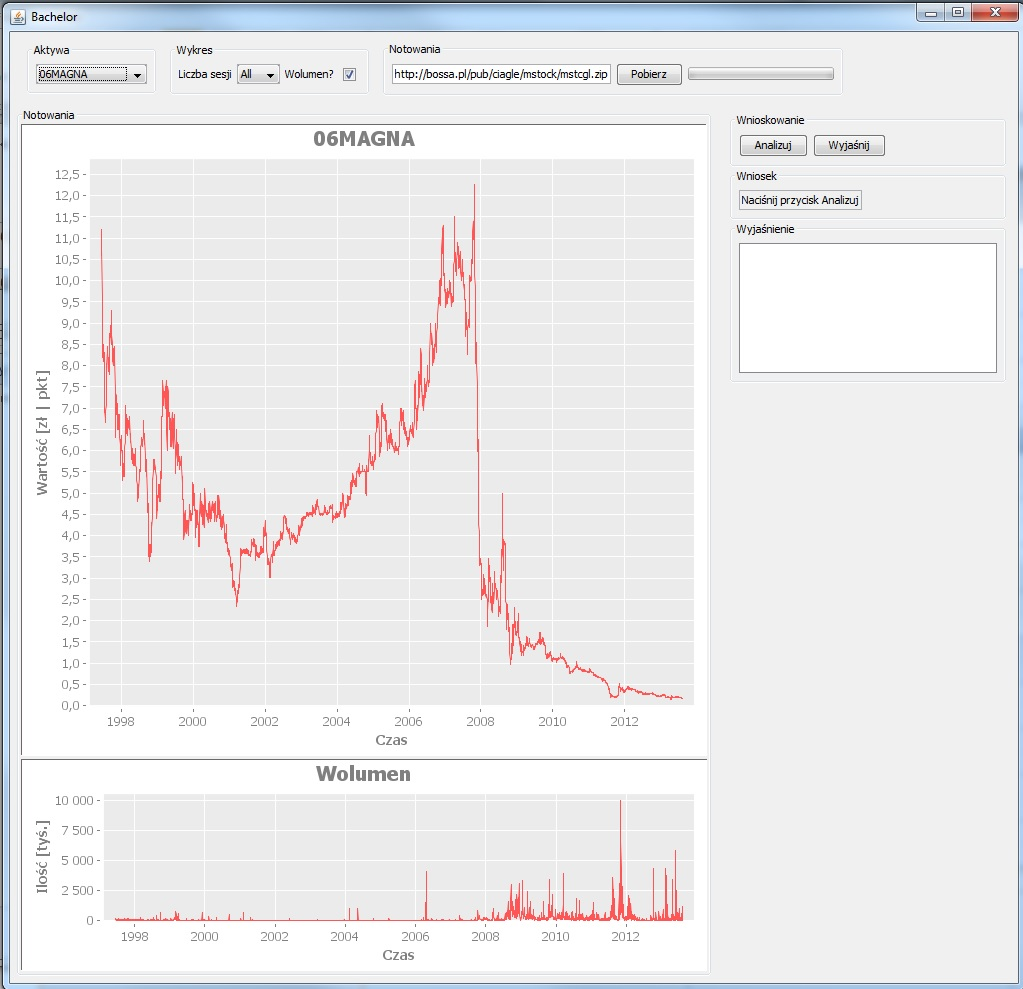
\includegraphics[width=0.9\textwidth]{1.jpg}
	\caption{Widok aplikacji po uruchomieniu}
	\label{fig:1}
\end{figure}

\subsection{Struktura projektu}

\paragraph{}
Projekt podzielony jest na 3 przestrzenie nazw:
\begin{itemize}
	\item bachelor.core
	\item bachelor.wsk
	\item bachelor.zip
\end{itemize}

\begin{tabular}{ c p{10,5cm}}
Przestrzeń nazw & Funkcjonalności \\ \hline \\
bachelor.core & Zawiera wszystkie funkcje parsera reguł, funkcje silnika wnioskującego, wczytywanie listy spółek, których dane znajdują się w~katalogu z~notowaniami. Tutaj również zdefiniowany jest interfejs użytkownika. Dodatkowo jest tu funkcja uruchamiająca wypakowywanie archiwum ZIP z~notowaniami \\
bachelor.wsk & Tutaj zdefiniowana jest funkcja wczytująca notowania z~pliku i~tworząca z~nich odpowiednią strukturę umieszczaną na liście notowań. W~tej przestrzeni nazw zdefiniowane są również wszystkie wskaźniki wykorzystywane przez system wnioskujący, a~także funkcje pomocnicze do wyliczania wskaźników i~operacji na liście notowań. Jest tu również umieszczona funkcja tworząca listy wszystkich zdefiniowanych wskaźników, a~także funkcje odwołujące się do tych list, które wykorzystywane są w~regułach. \\
bachelor.zip & Zdefiniowana jest tu funkcja do pobierania archiwum ze wskazanego adresu internetowego i~zapisu go na dysku. Znajdują się tu także wszystkie funkcje pomocnicze do rozpakowywania archiwum \\
\end{tabular}

\subsection{Gramatyka reguł}

\paragraph{}
Jedną z~funkcjonalności systemu jest parser reguł, które są wczytywane z~pliku tekstowego, a~następnie na ich podstawie generowany jest kod nowych funkcji, które przekazywane są do mechanizmu wnioskującego. Aby można było stworzyć taki parser najpierw trzeba było zaprojektować gramatykę, zgodnie z~którą można zapisywać reguły w~pliku tekstowym. Gramatyka ta ma następującą postać:\\
RULE = EXPR \textgreater\textgreater FACT \\
EXPR = (EXPR OpL EXPR) \textbar\space (WSK OpA NUM) \textbar\space (WSK OpA WSK) \textbar\space (FACT) \\
OpL = and \textbar\space or \\
OpA = \textgreater\space\textbar\space \textless \space\textbar\space == \\
WSK = [A-Z]+[A-Z0-9]* \\
FACT = [a-z]+[a-z0-9]* \\
NUM = [-+]?[0-9]+[.]?[0-9]*\textbar[0-9]+ \\

W~pierwszej kolejności linia z~regułą wczytana z~pliku parsowana jest przez bibliotekę Instaparse\cite{instaparse} do listy tokenów, czyli par opisanych jako
\begin{figure}[h]
	\centering 
	[:TYP\_TOKENA WARTOŚĆ]
\end{figure}

Następnie element z~listy o~typie :EXPR przekazywany jest do funkcji, która sprawdza, którym wariantem wyrażenia jest przekazany token. Na tej podstawie tworzy listę symboli możliwych do zinterpretowania przez Clojure, które odpowiadają funkcjonalnie treści wyrażenia. Utworzona lista symboli jest wykorzystywana jako ,,ciało'' funkcji przez makro, które generuje nowe funkcje reprezentujące reguły. Każde tak wygenerowane wyrażenie musi zwracać wartość logiczną prawda bądź fałsz. Podczas procesu wnioskowania zależnie od tej wartości do listy faktów dodawany jest nowy fakt, bądź mechanizm przechodzi do ewaluacji kolejnej funkcji - reguły.

Dzięki bibliotece Instaparse\cite{instaparse} w~łatwy sposób można powyższą gramatykę reguł przetworzyć na listę tokenów, a~z~takiej listy wygenerować funkcję, którą następnie można wywołać w~celu sprawdzenia, czy wszystkie przesłanki danej reguły są prawdziwe i~można dodać nowy fakt do bazy wiedzy.

\lstset{language=Lisp,
	breaklines=true,
	keywordstyle=\color{blue},
	morekeywords={def,defn},
	stringstyle=\color{red},
	numbers=left,
	numbersep=5pt,
	showspaces=false,
	showtabs=false,
	showstringspaces=false,
	captionpos=b,
	caption={Zdefiniowana gramatyka wykorzystywania do tworzenia listy tokenów z reguły}}
\begin{lstlisting}
(def grammar
  (insta/parser
    "RULE = EXPR' >> 'FACT
     EXPR = '('EXPR' 'OpL' 'EXPR')' | '('WSK' 'OpA' 'NUM')' | '('WSK' 'OpA' 'WSK')' | '('FACT')'
     OpL = 'and' | 'or'
     OpA = '>' | '<' | '=='
     WSK = #'[A-Z]+[A-Z0-9]*'
     FACT = #'[a-z]+[a-z0-9]*'
     NUM = #'[-+]?[0-9]+[.]?[0-9]*|[0-9]+'")
  )
\end{lstlisting}

\lstset{language=Lisp,
	breaklines=true,
	keywordstyle=\color{blue},
	morekeywords={def,defn},
	stringstyle=\color{red},
	numbers=left,
	numbersep=5pt,
	showspaces=false,
	showtabs=false,
	showstringspaces=false,
	captionpos=b,
	caption={Makro generujące funkcję - wykorzystuje listę tokenów}}
\begin{lstlisting}
(defmacro generate-funcs 
  "creates function from parse-tree"
  [parse-tree]
  (let [[_ expr _ [_ fact-value]] parse-tree
        arg (gensym "facts")
        expression (parse-expr expr arg)
        new-fact (str fact-value)]
    `(fn 
       [~arg] 
       (if ~expression
         (str ~new-fact) 
         ())
       )
    )
  )
\end{lstlisting}

\pagebreak

\lstset{language=Lisp,
	breaklines=true,
	keywordstyle=\color{blue},
	morekeywords={def,defn},
	stringstyle=\color{red},
	numbers=left,
	numbersep=5pt,
	showspaces=false,
	showtabs=false,
	showstringspaces=false,
	captionpos=b,
	caption={Funkcja tworząca ,,ciało'' funkcji z listy tokenów}}
\begin{lstlisting}
(defn parse-expr 
  "parses expr struct into list of symbols"
  [expr arg]
  (cond
    (empty? expr) ()
    :else
    (let [[_ _ [part1-type part1-val] _ [part2-type part2-val] _ [part3-type part3-val] _] expr]
      (cond 
        (and (= :WSK part1-type) (= :OpA part2-type) (= :NUM part3-type)) 
	(let 
	 [wsk (symbol (str "bachelor.wsk/" part1-val))
	 opa (symbol part2-val)
	 num (Integer/valueOf part3-val)]
	 (list opa (list wsk) num))
        (and (= :WSK part1-type) (= :OpA part2-type) (= :WSK part3-type)) 
	(let
	 [wsk1 (symbol (str "bachelor.wsk/" part1-val))
	 opa (symbol part2-val)
	 wsk2 (symbol (str "bachelor.wsk/" part3-val))]
	 (list opa (list wsk1) (list wsk2)))
        (= :OpL part2-type) 
	(let
	 [expr1 (parse-expr (get expr 2) arg)
	 opl (symbol part2-val)
	 expr2 (parse-expr (get expr 6) arg)]
	 (list opl expr1 expr2))
        (= :FACT part1-type) 
	(let
	 [fact (str part1-val)
	 bool (symbol "boolean")
	 some (symbol "some")]
	 (list bool (list some #{fact} arg)))
        :else
        ())
      )
    )
  )
\end{lstlisting}

\subsection{Mechanizm wnioskujący}

\paragraph{}
Silnik wnioskujący opiera się o~wnioskowanie w~przód i~składa się z~dwóch funkcji. Pierwsza z~nich cyklicznie wywołuje drugą, przekazując do niej listę reguł i~aktualną listę faktów. Druga funkcja uruchamia kolejno wszystkie reguły. Jeśli można uruchomić regułę i~wartość logiczne jej wyrażenia to prawda, wtedy sprawdzane jest czy na liście faktów znajduje się już fakt generowany przez tą regułę. Jeśli nie, jest on dodawany i~uruchamiana jest kolejna reguła. Po każdym wykonaniu funkcji sprawdzającej wszystkie reguły, główna funkcja wnioskująca sprawdza, czy na liście faktów pojawił się fakt mówiący o~tym aby kupić bądź sprzedać dane akcje. Dodatkowo sprawdza też, czy zmieniła się liczba wygenerowanych faktów. Jeśli nie, oznacza to, że~nie można uruchomić już żadnej nowej reguły i~nie da się uzyskać wniosku kupuj bądź sprzedaj.

\lstset{language=Lisp,
	breaklines=true,
	keywordstyle=\color{blue},
	morekeywords={def,defn},
	stringstyle=\color{red},
	numbers=left,
	numbersep=5pt,
	showspaces=false,
	showtabs=false,
	showstringspaces=false,
	captionpos=b,
	caption={Główna funkcja wnioskująca}}
\begin{lstlisting}
(defn inference
  "evaluates all rules as long as don't get buy or sell conclusion"
  [rules facts]
  (cond
    (done? facts) facts
    (empty? rules) facts
    (= (count facts) (count (vec (evaluateRules rules facts)))) facts
    :else
    (inference rules (vec (evaluateRules rules facts))))
  )
\end{lstlisting}

\lstset{language=Lisp,
	breaklines=true,
	keywordstyle=\color{blue},
	morekeywords={def,defn},
	stringstyle=\color{red},
	numbers=left,
	numbersep=5pt,
	showspaces=false,
	showtabs=false,
	showstringspaces=false,
	captionpos=b,
	caption={Funkcja sprawdzająca wszystkie reguły}}
\begin{lstlisting}
(defn evaluateRules
  "evaluates rules"
  [rules facts]
  (cond
    (empty? rules) facts
    (empty? (eval (list (first rules) facts))) (evaluateRules (rest rules) facts)
    (containsFact? (eval (list (first rules) facts)) facts) (evaluateRules (rest rules) facts)
    :else
    (cons (eval (list (first rules) facts)) (evaluateRules (rest rules) facts)))
  )
\end{lstlisting}

\begin{figure}[H]
	\centering
	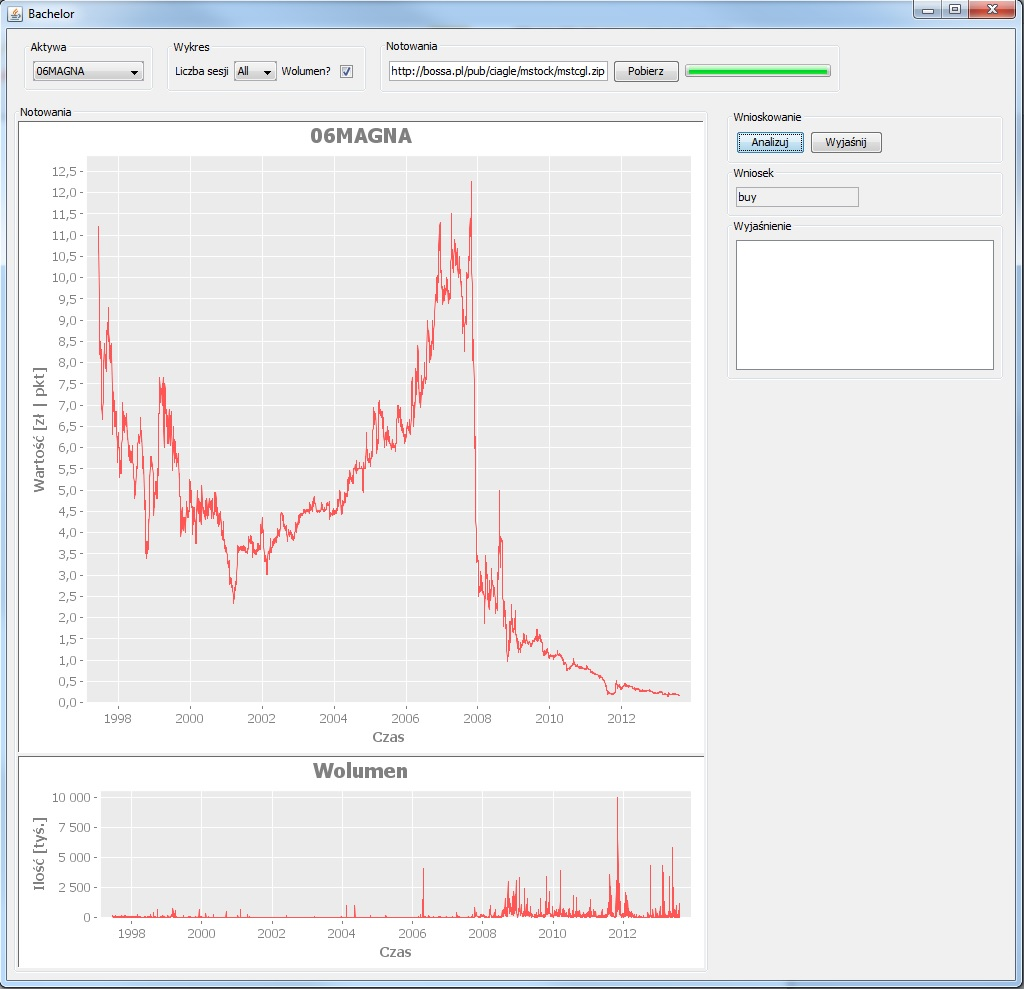
\includegraphics[width=0.9\textwidth]{4.jpg}
	\caption{Analiza notowań spółki}
	\label{fig:4}
\end{figure}

\begin{figure}[H]
	\centering
	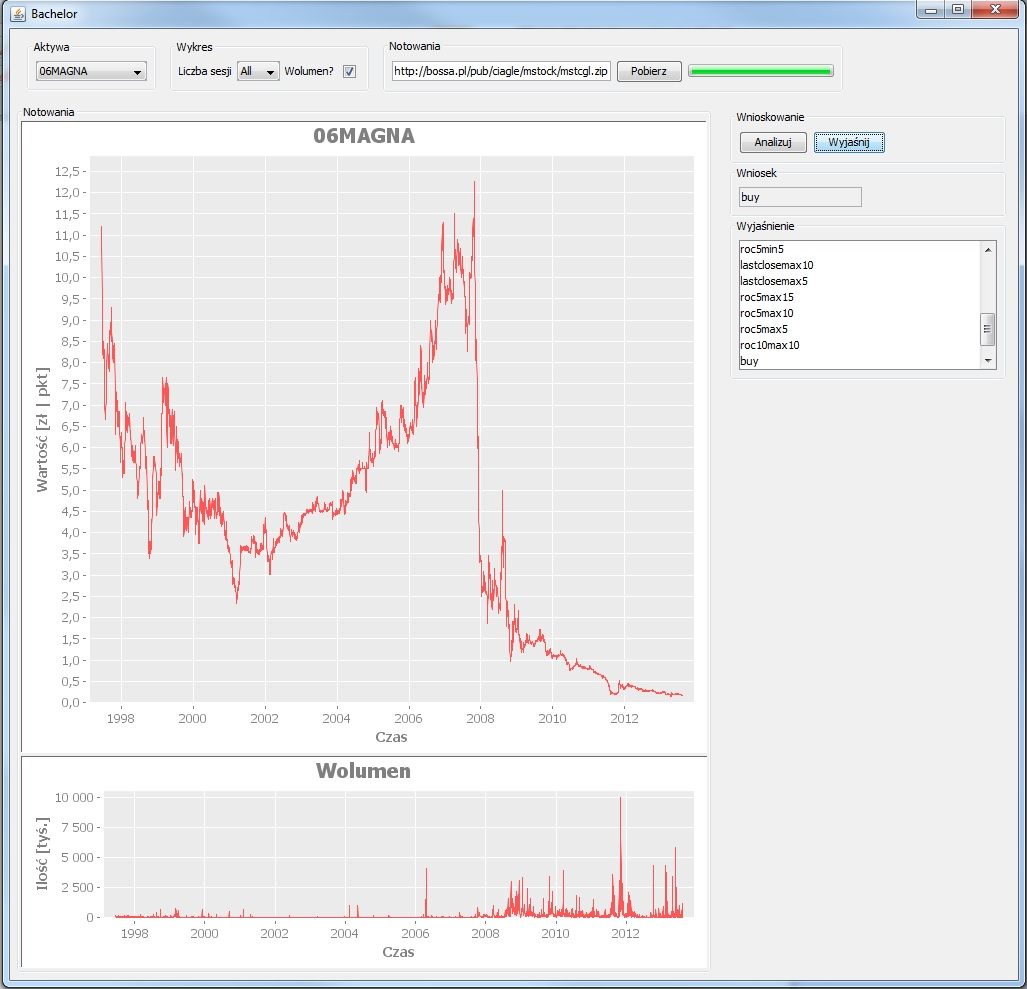
\includegraphics[width=0.9\textwidth]{5.jpg}
	\caption{Przedstawienie listy wygenerowanych faktów podczas wnioskowania - wariant z wnioskiem kupuj}
	\label{fig:5}
\end{figure}

\begin{figure}[H]
	\centering
	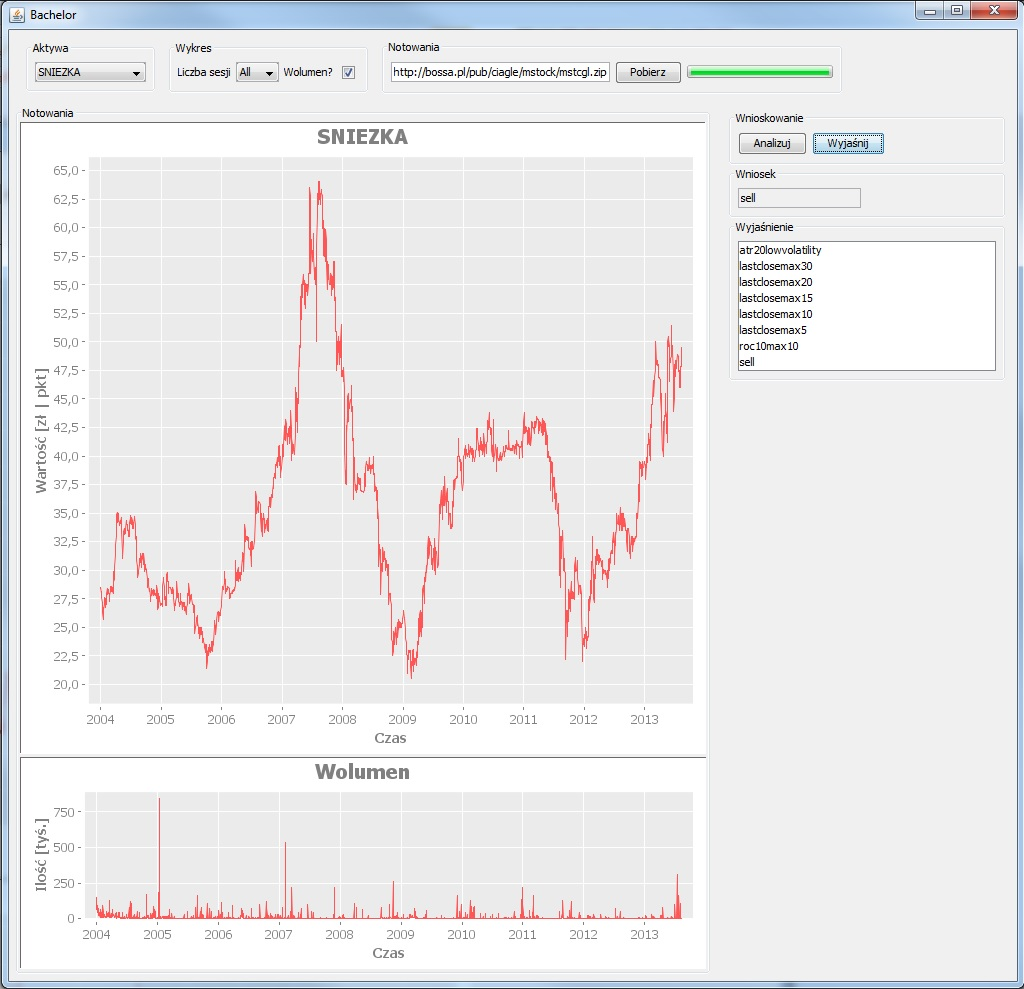
\includegraphics[width=0.9\textwidth]{7.jpg}
	\caption{Przedstawienie listy wygenerowanych faktów podczas wnioskowania - wariant z wnioskiem sprzedaj}
	\label{fig:2}
\end{figure}

\begin{figure}[H]
	\centering
	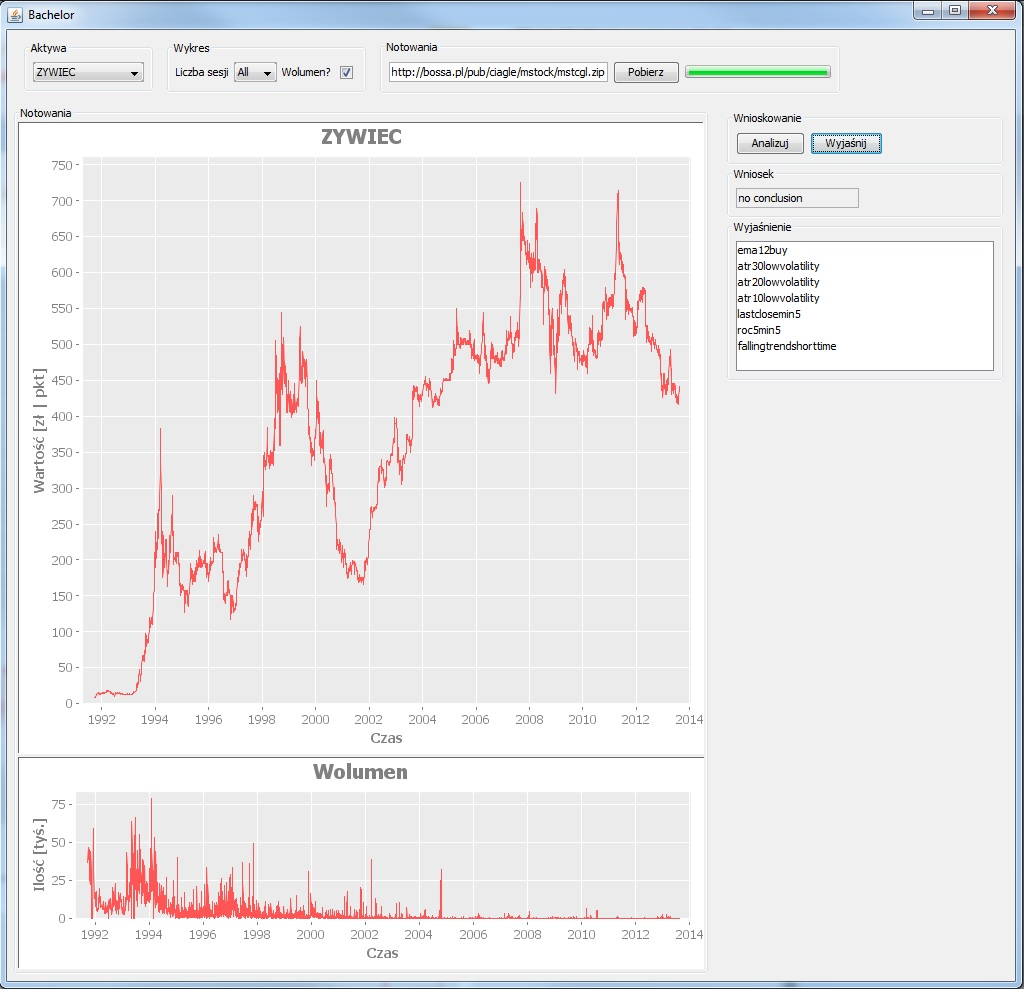
\includegraphics[width=0.9\textwidth]{6.jpg}
	\caption{Przedstawienie listy wygenerowanych faktów podczas wnioskowania - wariant przy braku wniosków}
	\label{fig:6}
\end{figure}

\subsection{Obsługa plików ZIP}

\paragraph{}
Archiwum ZIP z~notowaniami spółek z~GPW w~Warszawie obsługiwane jest w~przestrzeni nazw bachelor.zip. Po naciśnięciu przycisku Pobierz wywoływana jest funkcja, która pobiera plik ZIP ze~wskazanego w~polu tekstowym adresu www. Następnie ścieżka do zapisanego pliku przekazywana jest do głównej funkcji rozpakowującej. Funkcja ta dla każdego elementu z~archiwum tworzy nowy plik z~nazwą tego elementu, a~następnie zapisuje do niego tablicę bajtów z~zawartością tego pliku. Ze~względu na obsługę paska postępu wykonywanych operacji, główna funkcja wnioskująca znajduje się w~głównej przestrzeni nazw, a~wszystkie funkcje pomocnicze w~przestrzeni bachelor.zip. Cały proces pobierania i~rozpakowywania archiwum odbywa się w~osobnym wątku, tak aby nie blokować działania reszty interfejsu użytkownika.
\pagebreak

\lstset{language=Lisp,
	breaklines=true,
	keywordstyle=\color{blue},
	morekeywords={def,defn},
	stringstyle=\color{red},
	numbers=left,
	numbersep=5pt,
	showspaces=false,
	showtabs=false,
	showstringspaces=false,
	captionpos=b,
	caption={Funkcja zapisująca pojedynczy plik z archiwum}}
\begin{lstlisting}
(defn writeZipEntry
  "Writes zip entry to file"
  [zip entry]
  (with-open [w (io/writer (str "resources/notowania/" (.getName entry)))]
     (.write w (getZipEntryContent zip entry)))
  )
\end{lstlisting}

\lstset{language=Lisp,
	breaklines=true,
	keywordstyle=\color{blue},
	morekeywords={def,defn},
	stringstyle=\color{red},
	numbers=left,
	numbersep=5pt,
	showspaces=false,
	showtabs=false,
	showstringspaces=false,
	captionpos=b,
	caption={Funkcja odczytująca zawartość pojedynczego pliku z archiwum}}
\begin{lstlisting}
(defn getZipEntryContent
  "Reads zip entry content"
  [zip entry]
  (slurp (.getInputStream zip entry))
  )
\end{lstlisting}

\begin{figure}[H]
	\centering
	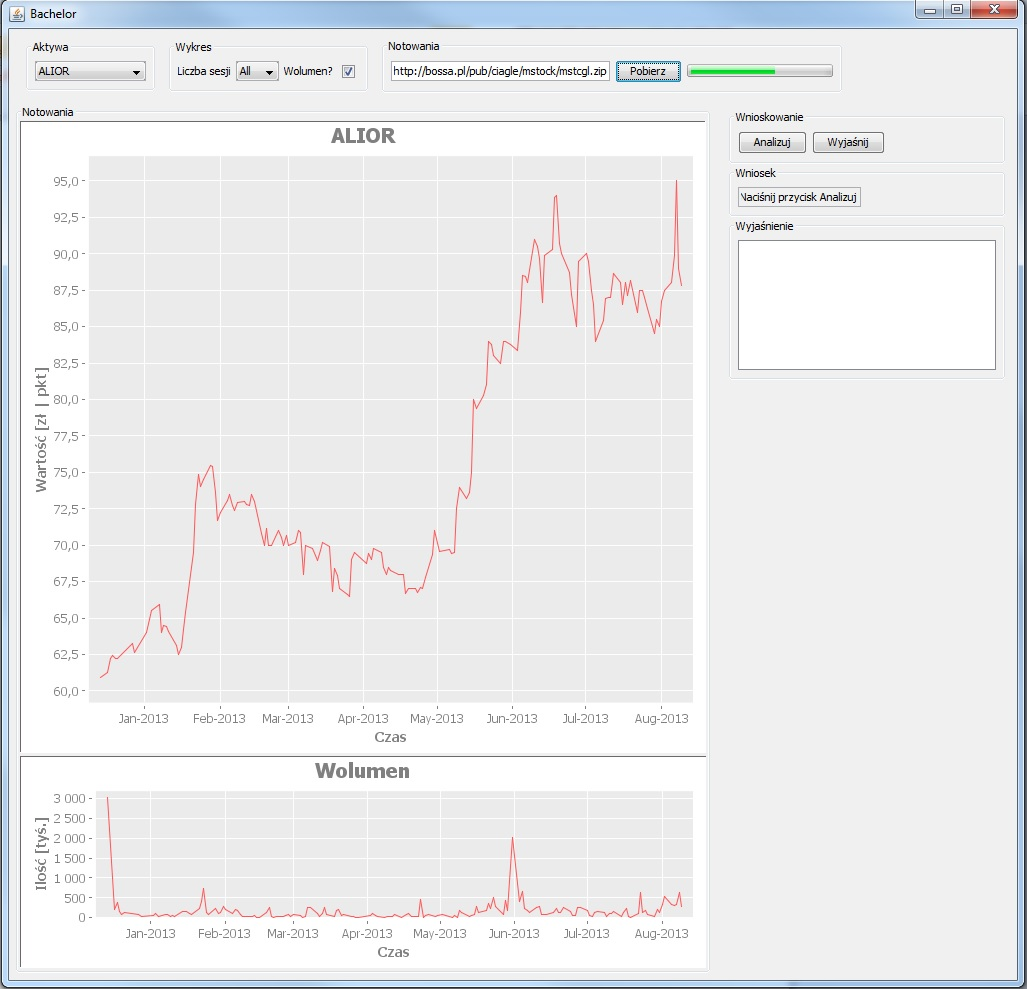
\includegraphics[width=0.9\textwidth]{2.jpg}
	\caption{Pobieranie nowych notowań}
	\label{fig:2}
\end{figure}

\begin{figure}[H]
	\centering
	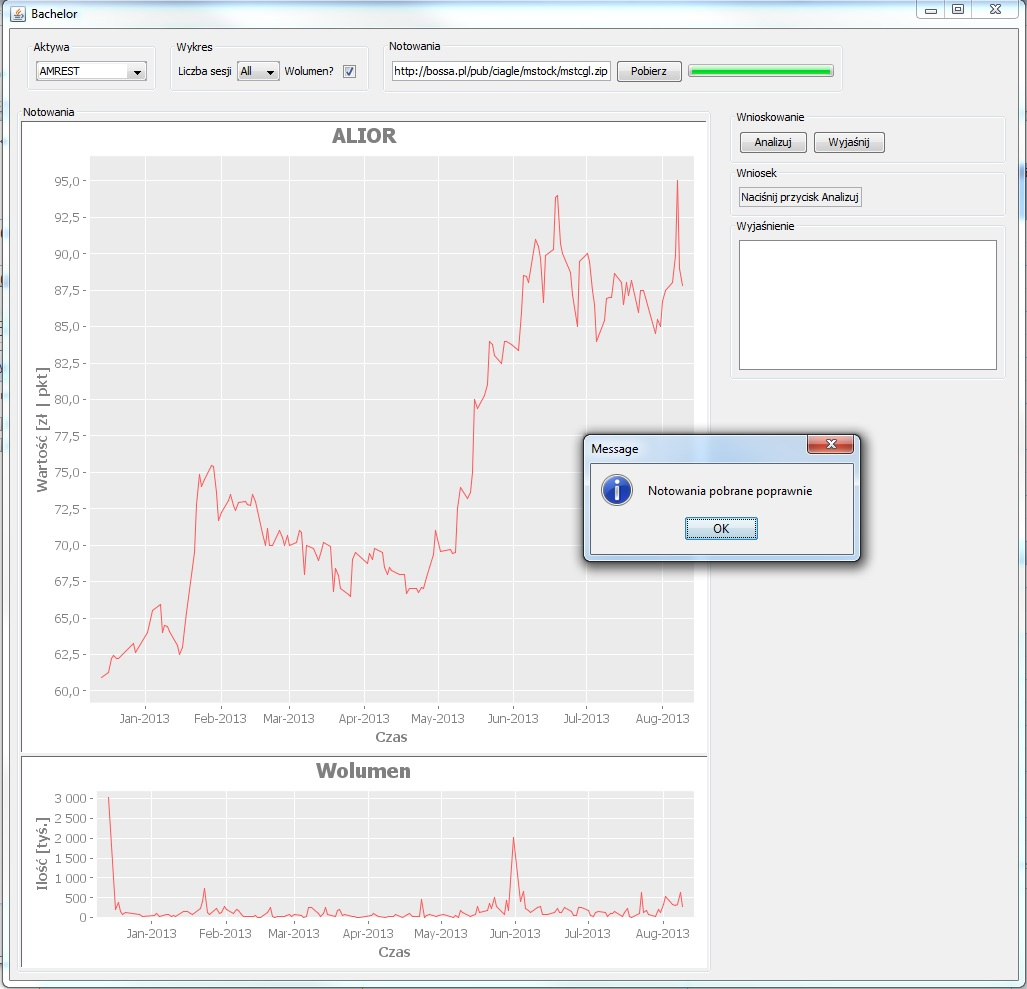
\includegraphics[width=0.9\textwidth]{3.jpg}
	\caption{Poprawne pobranie i rozpakowanie nowych notowań}
	\label{fig:3}
\end{figure}

\subsection{Struktura danych o~notowaniach}

\paragraph{}
Dane o~notowaniach spółek giełdowych, które wczytywane są z~pliku, w~aplikacji przechowywane są w~następującej strukturze:
\begin{description} 
	\item[Company] \hfill
		\begin{itemize}
			\item Name - nazwa spółki
			\item \begin{description}
					\item[Session] \hfill
						\begin{itemize}
							\item Date - data sesji
							\item Open - cena otwarcia sesji
							\item High - cena maksymalna podczas sesji
							\item Low - cena minimalna podczas sesji
							\item Close - cena zamknięcia sesji
							\item Vol - wolumen
						\end{itemize}
				\end{description}
		\end{itemize}
\end{description}

\lstset{language=Lisp,
	breaklines=true,
	keywordstyle=\color{blue},
	morekeywords={def,defn},
	deletekeywords={open,close},
	stringstyle=\color{red},
	numbers=left,
	numbersep=5pt,
	showspaces=false,
	showtabs=false,
	showstringspaces=false,
	captionpos=b,
	caption={Struktura notowań zdefiniowana w języku Clojure}}
\begin{lstlisting}
(defstruct Company :name :session)

(defstruct Session :date :open :high :low :close :vol)
\end{lstlisting}

\subsection{Wykresy}

\paragraph{}
W~aplikacji została wykorzystana biblioteka Incanter\cite{incanter} pozwalająca generować wykresy z~dostarczonych struktur danych. Wykorzystywany jest jedynie szablon wykresów czasowych, do~którego przekazujemy listę dat jako wartości dla osi poziomej i~drugą listę z~wartościami dla osi pionowej. Domyślnie rysowane są dwa wykresy:
\begin{itemize}
	\item Wartości akcji (indeksu) - główny wykres przedstawiający cenę akcji wybranej spółki, bądź wartość wybranego indeksu
	\item Wolumenu - dodatkowy wykres prezentujący wartość wolumenu
\end{itemize}

\lstset{language=Lisp,
	breaklines=true,
	keywordstyle=\color{blue},
	morekeywords={def,defn},
	stringstyle=\color{red},
	numbers=left,
	numbersep=5pt,
	showspaces=false,
	showtabs=false,
	showstringspaces=false,
	captionpos=b,
	caption={Przykładowa funkcja rysująca wykres przy pomocy biblioteki Incanter\cite{incanter}}}
\begin{lstlisting}
(ChartPanel. 
  (charts/time-series-plot 
    (x (read-string (config sessions :text)) (wsk/createCompany (config companiesList :text))) 
    (y (read-string (config sessions :text)) (wsk/createCompany (config companiesList :text)))
    :title (config companiesList :text)
    :x-label "Czas"
    :y-label "Wartosc [zl | pkt]"))
\end{lstlisting}

Istnieje możliwość ukrycia wykresu wolumenu, a~także wyboru z~rozwijanej listy dla ilu sesji mają być rysowane wykresy.

\begin{figure}[H]
	\centering
	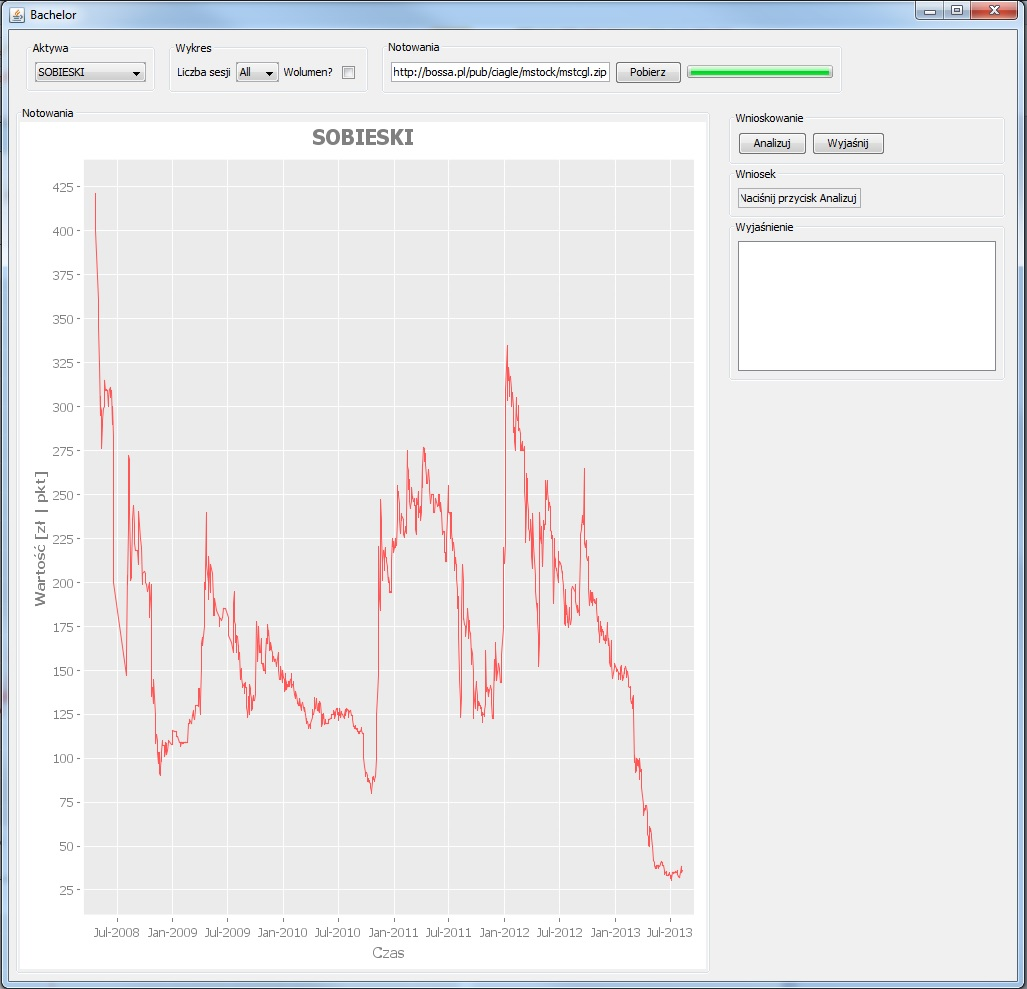
\includegraphics[width=0.9\textwidth]{8.jpg}
	\caption{Widok z ukrytym wykresem wolumenu}
	\label{fig:8}
\end{figure}

\begin{figure}[H]
	\centering
	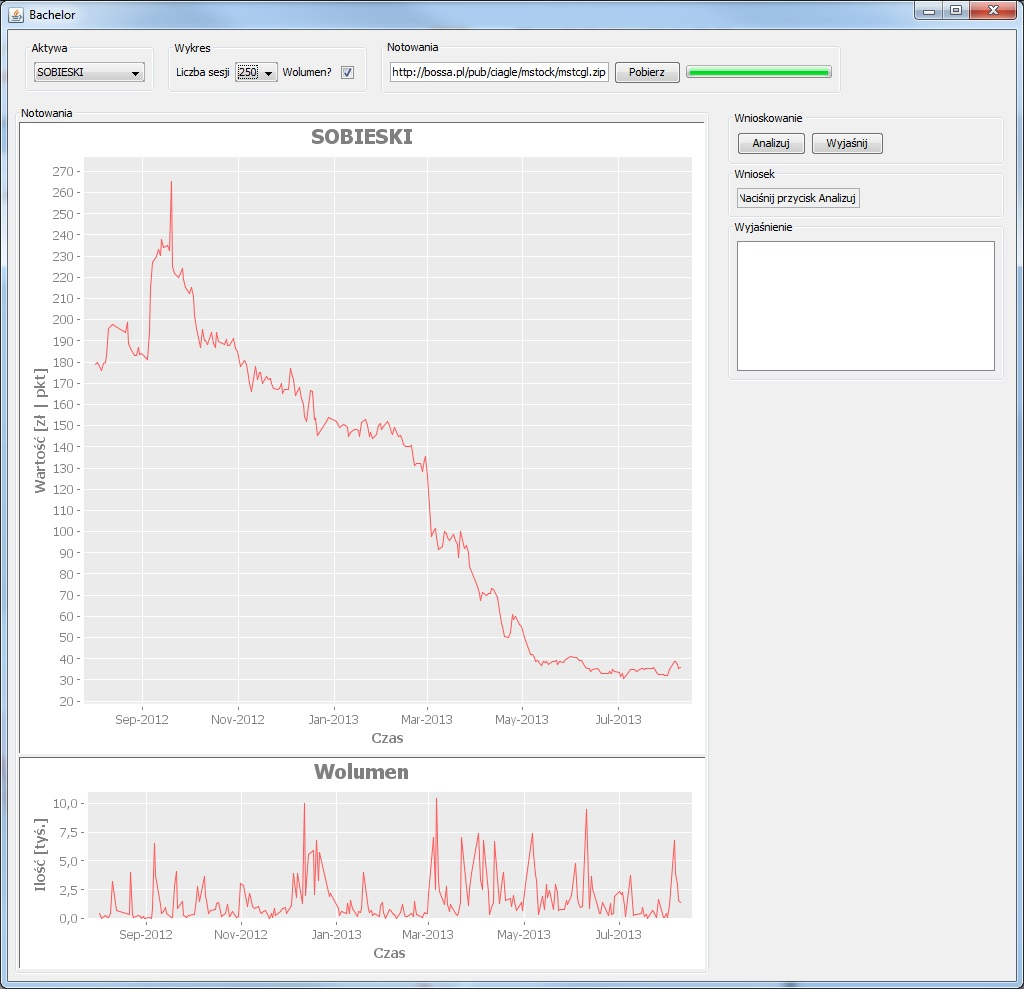
\includegraphics[width=0.9\textwidth]{9.jpg}
	\caption{Widok wykresów dla 250 ostatnich sesji}
	\label{fig:9}
\end{figure}

\begin{figure}[H]
	\centering
	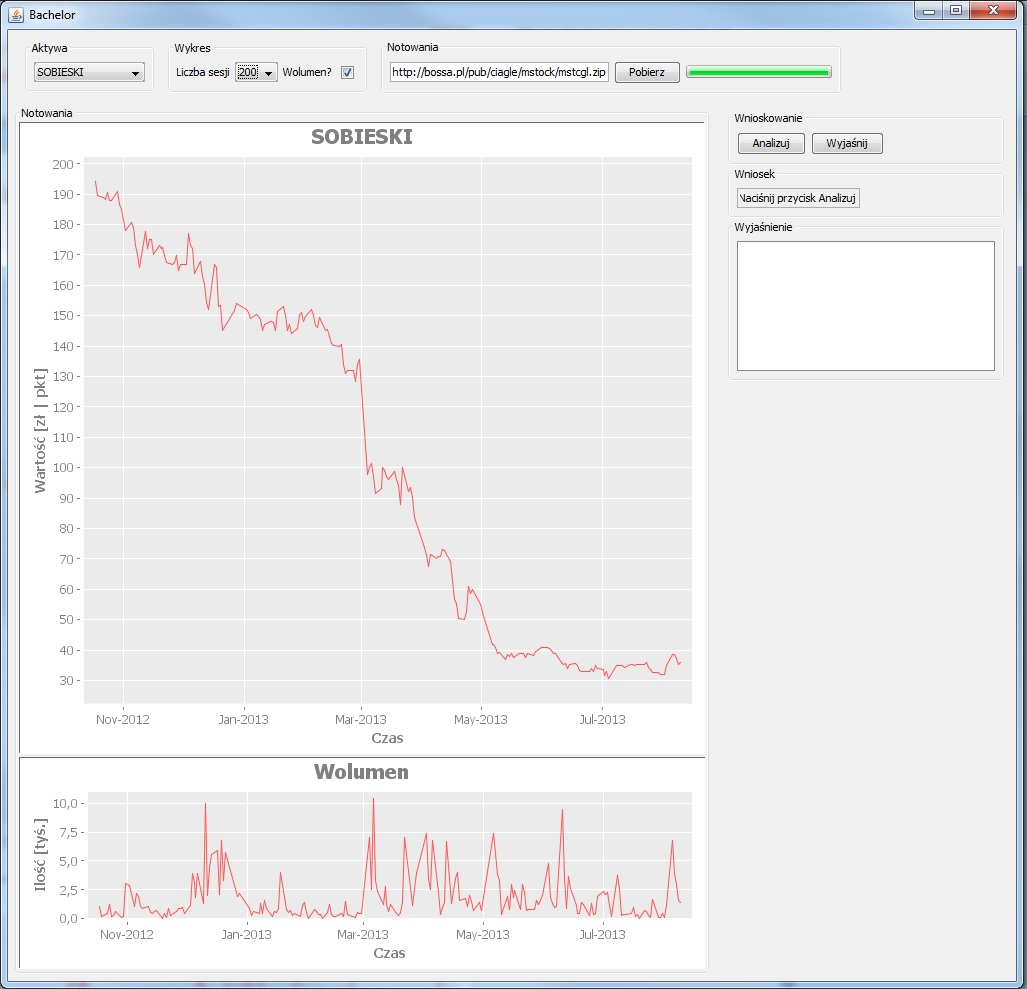
\includegraphics[width=0.9\textwidth]{10.jpg}
	\caption{Widok wykresów dla 200 ostatnich sesji}
	\label{fig:10}
\end{figure}

\begin{figure}[H]
	\centering
	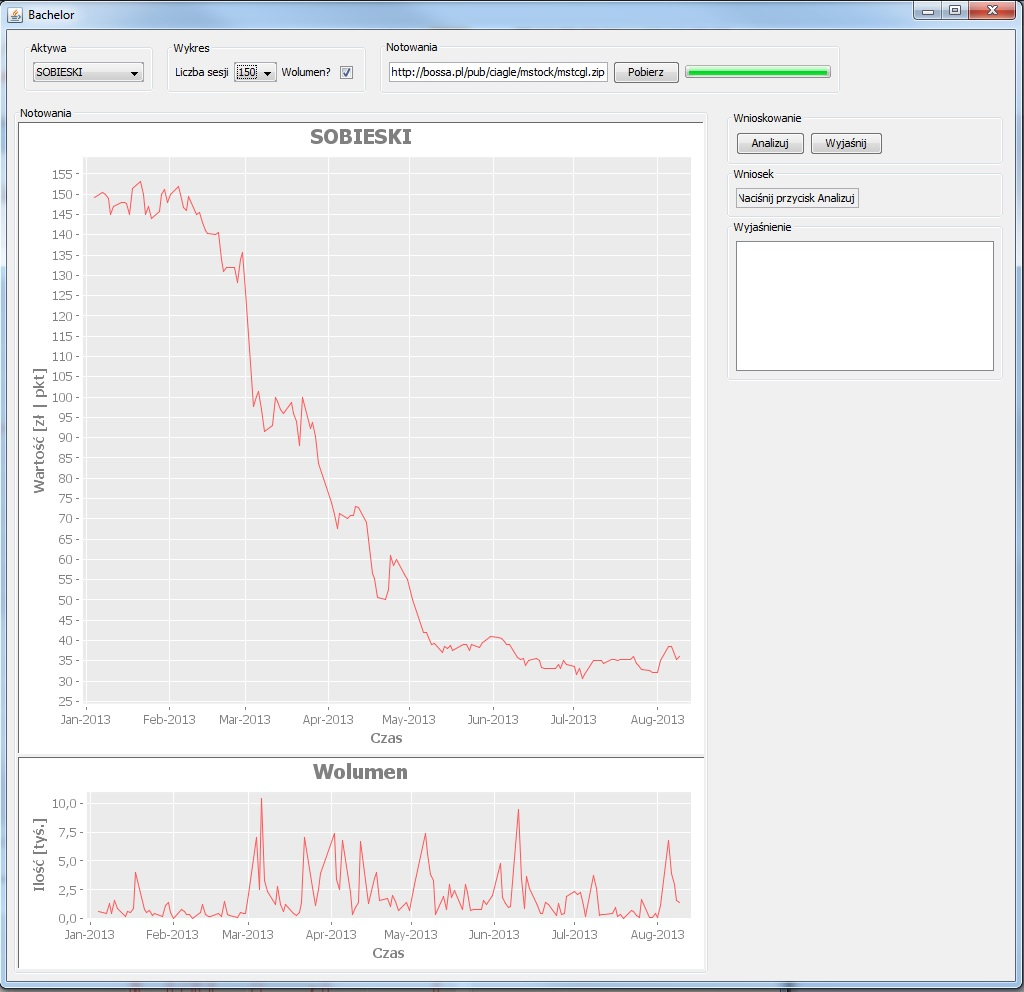
\includegraphics[width=0.9\textwidth]{11.jpg}
	\caption{Widok wykresów dla 150 ostatnich sesji}
	\label{fig:11}
\end{figure}

\begin{figure}[H]
	\centering
	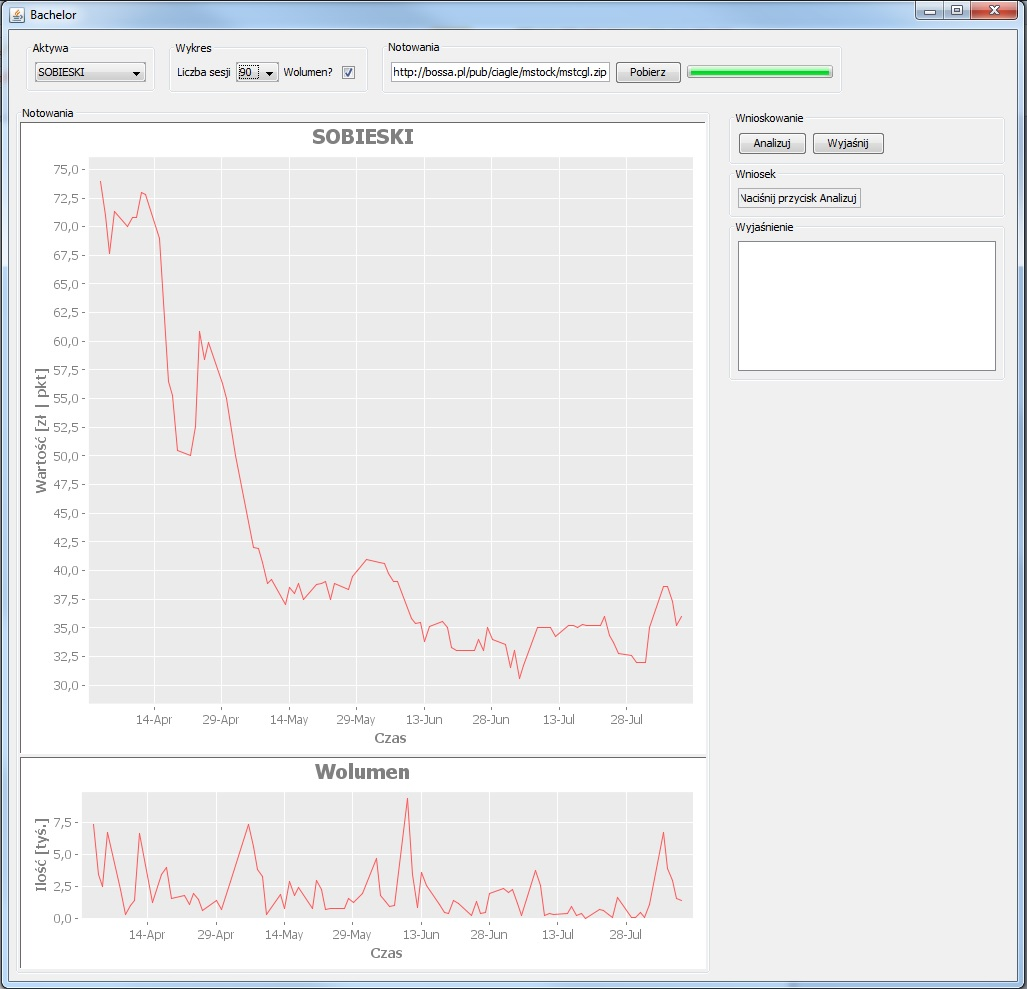
\includegraphics[width=0.9\textwidth]{12.jpg}
	\caption{Widok wykresów dla 90 ostatnich sesji}
	\label{fig:12}
\end{figure}

\begin{figure}[H]
	\centering
	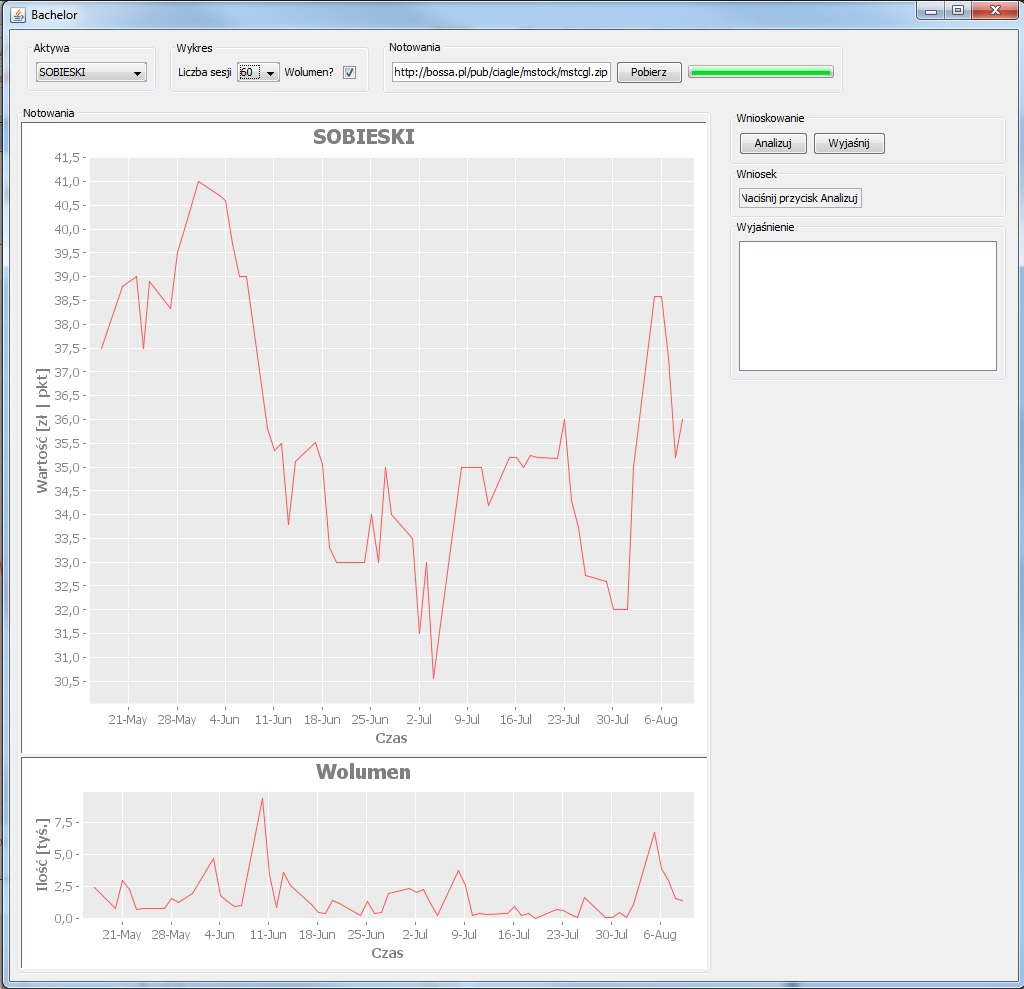
\includegraphics[width=0.9\textwidth]{13.jpg}
	\caption{Widok wykresów dla 60 ostatnich sesji}
	\label{fig:13}
\end{figure}

\begin{figure}[H]
	\centering
	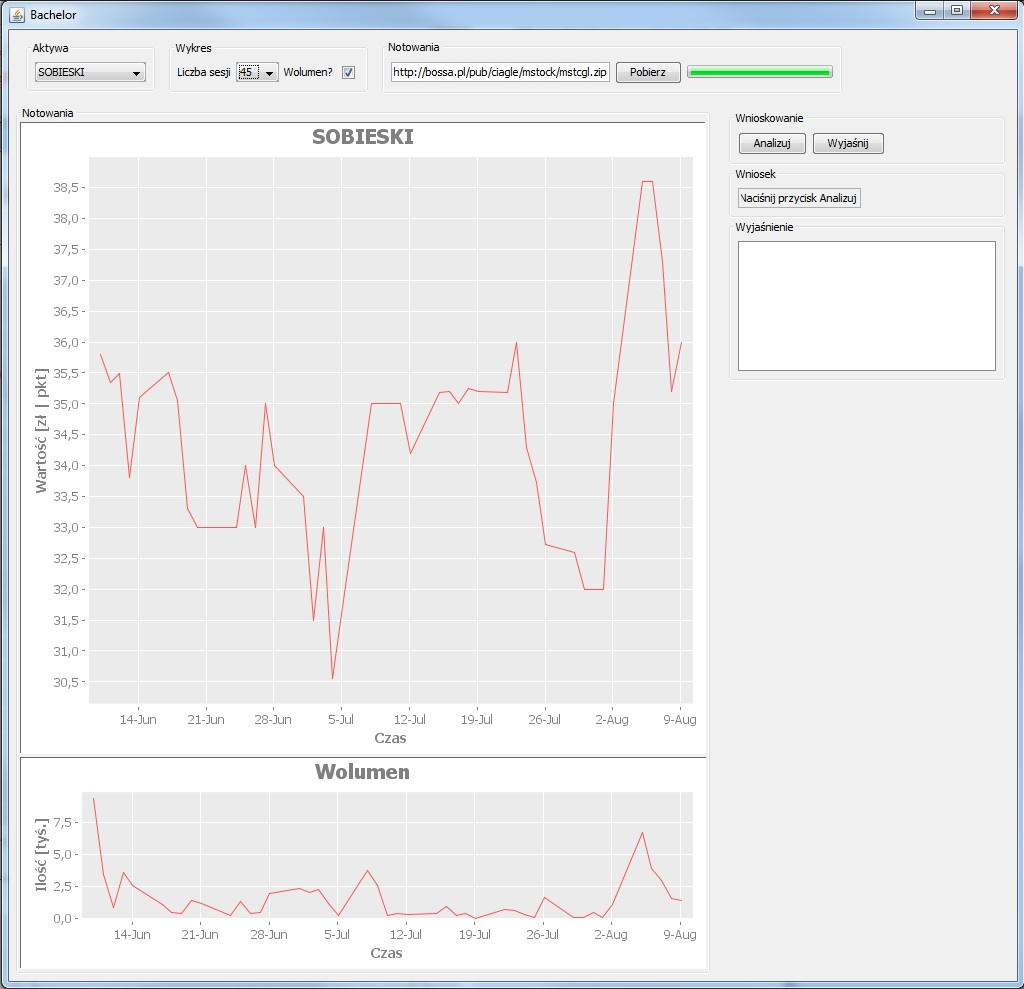
\includegraphics[width=0.9\textwidth]{14.jpg}
	\caption{Widok wykresów dla 45 ostatnich sesji}
	\label{fig:14}
\end{figure}

\begin{figure}[H]
	\centering
	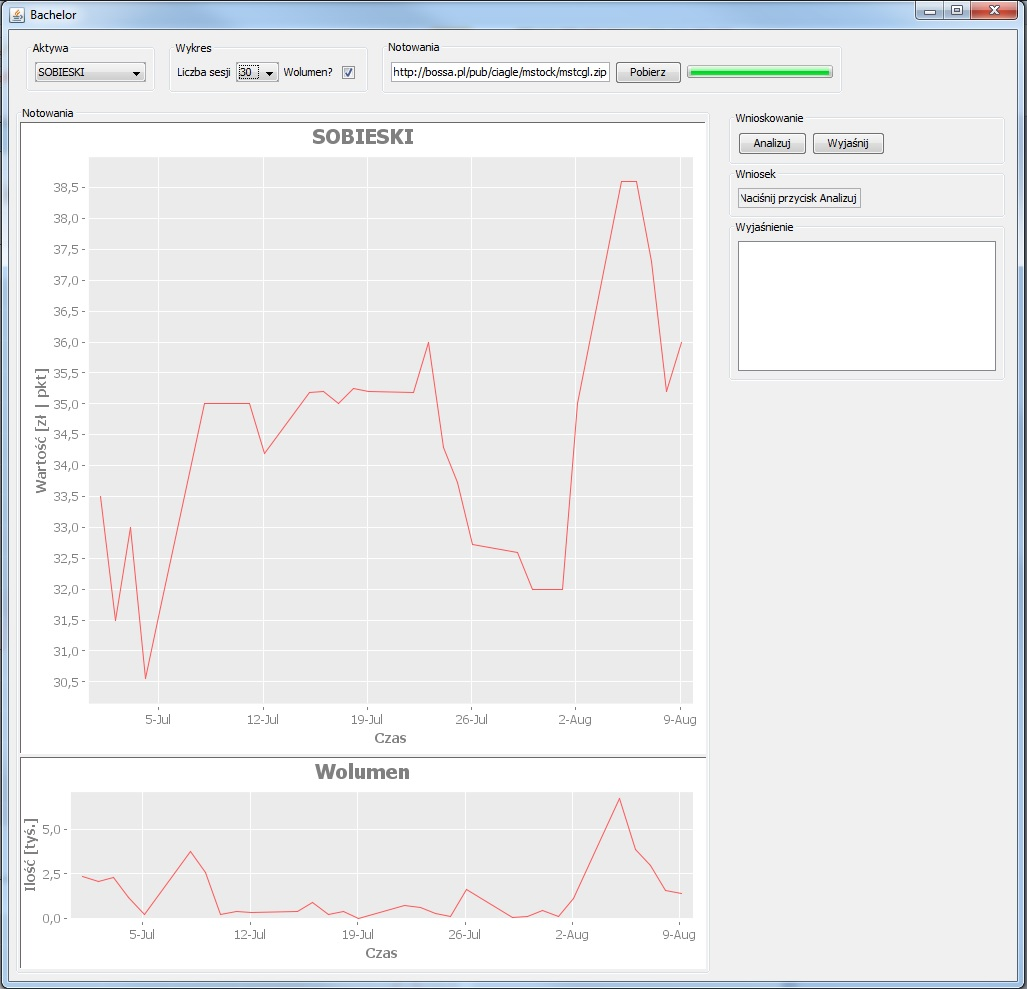
\includegraphics[width=0.9\textwidth]{15.jpg}
	\caption{Widok wykresów dla 30 ostatnich sesji}
	\label{fig:15}
\end{figure}

\begin{figure}[H]
	\centering
	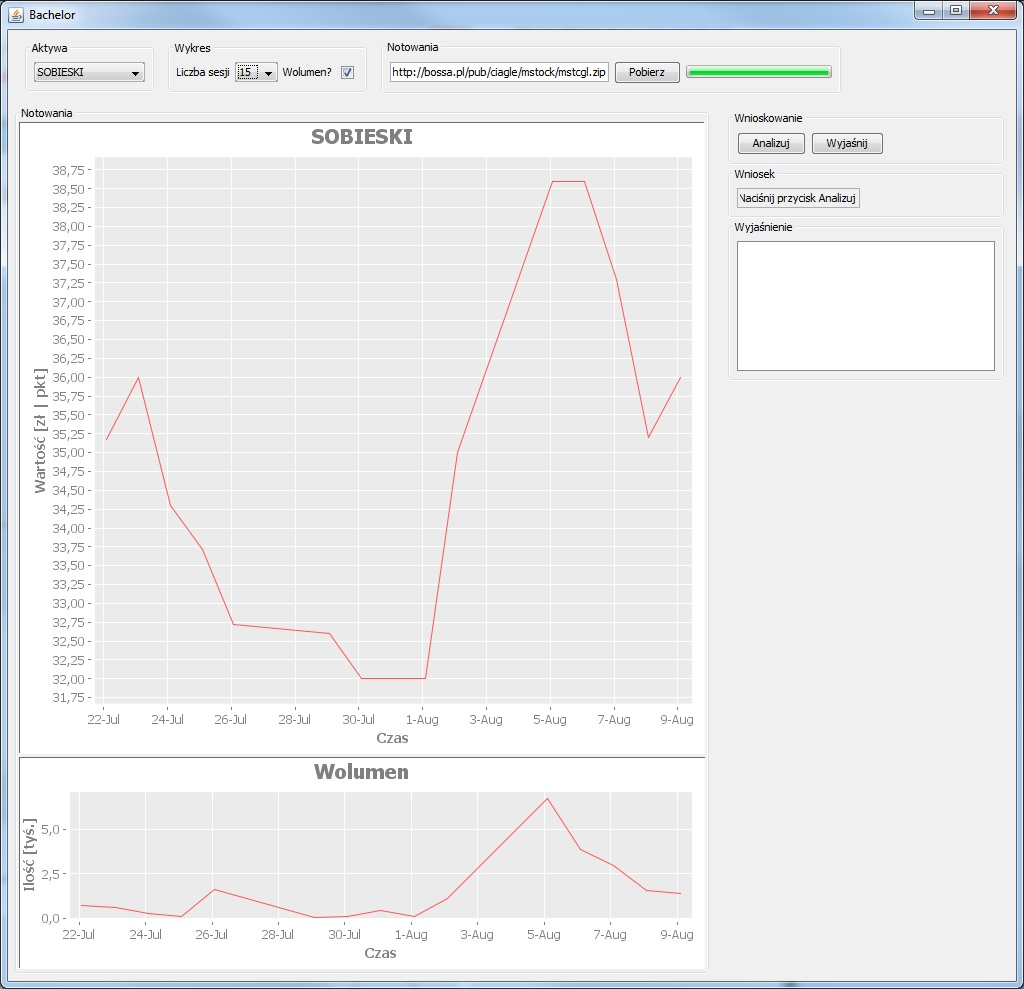
\includegraphics[width=0.9\textwidth]{16.jpg}
	\caption{Widok wykresów dla 15 ostatnich sesji}
	\label{fig:16}
\end{figure}

\subsection{Obliczane wskaźniki analizy technicznej}

\paragraph{}
Podczas procesu wnioskowania wykorzystywanych jest wiele wskaźników analizy technicznej. Poniżej znajduje się lista tych wskaźników wraz ze~sposobem ich obliczania:
\begin{description}
	\item[MFI] - Money Flow Index \hfill \\
		$\displaystyle MFI = 100 \times { pozytywny\ money\ flow \over pozytywny \ money \ flow + negatywny\ money\ flow }$  \hfill \\
			, gdzie \hfill
				\begin{itemize}
					\item ,,pozytywny money flow'' jest sumą {\textit{money flow}} z~dni, w~których cena typowa przewyższała cenę typową z~dnia poprzedniego
					\item ,,negatywny money flow'' jest sumą {\textit{money flow}} z~dni, w~których cena typowa była niższa niż w~dniu poprzednim
					\item $\displaystyle money \ flow = cena \ typowa \times wolumen$
					\item $\displaystyle cena\ typowa = {cena \ maksymalna + cena \ minimalna + cena \ zamkniecia \over 3}$
				\end{itemize}
	\item[ATR] - Average True Range \hfill \\
		Jest to średnia arytmetyczna z rzeczywistego zakresu zmian (ang. TR - True Range) dla zadanej liczby sesji. TR to największa co do modułu wartość z:
		\begin{itemize}
			\item różnicy między ceną najwyższą i~najniższą podczas analizowanej sesji
			\item różnicy między ceną zamknięcia sesji poprzedzającej analizowaną sesję a~ceną najwyższą podczas analizowanej sesji
			\item różnicy między ceną zamknięcia sesji poprzedzającej analizowaną sesję a~ceną najniższą podczas analizowanej sesji
		\end{itemize}
	\item[ROC] - Wskaźnik zmiany ROC (ang. Rate of Change) \hfill \\
		$\displaystyle ROC(n, k) = { C_n - C_{n-k} \over C_{n-k} } \times 100\%$ \\
		, gdzie \hfill
			\begin{itemize}
				\item C - cena zamknięcia
				\item n - numer analizowanej sesji
				\item k - liczba sesji wstecz w~odniesieniu do obecnie analizowanej
			\end{itemize}
	\item[Momentum] \hfill \\
		$\displaystyle Momentum(n, k) = C_n - C_{n-k}$ \\
		, gdzie \hfill
			\begin{itemize}
				\item C - cena zamknięcia
				\item n - numer analizowanej sesji
				\item k - liczba sesji wstecz w~odniesieniu do obecnie analizowanej
			\end{itemize}
	\item[SMA] - Prosta średnia krocząca (ang. Simple moving average) \hfill \\
		$\displaystyle \textit{SMA} = { C_{0} + C_{1} + \cdots + C_{n-1} \over n }$ \\
		, gdzie \hfill
			\begin{itemize}
				\item C - cena zamknięcia
				\item n - liczba analizowanych sesji
			\end{itemize}
	\item[WMA] - Ważona średnia krocząca (ang. Weighted moving average) \hfill \\
		$\displaystyle \textit{WMA} = { n C_{0} + (n-1) C_{1} + \cdots + C_{n-1} \over n + (n-1) + \cdots + 2 + 1}$ \\
		, gdzie \hfill
			\begin{itemize}
				\item C - cena zamknięcia
				\item n - liczba analizowanych sesji, a~zarazem wagi kolejnych okresów
			\end{itemize}
	\item[EMA] - Wykładnicza średnia krocząca (ang. Expotencial moving average) \hfill \\
		$\displaystyle \textit{EMA} = { C_0 + (1-\alpha) C_1 + (1-\alpha)^2 C_2 + (1-\alpha)^3 C_3 + \cdots + (1-\alpha)^n C_n \over 1 + (1-\alpha) + (1-\alpha)^2 + (1-\alpha)^3 + \cdots + (1-\alpha)^n}$ \\
		, gdzie \hfill
			\begin{itemize}
				\item C - cena zamknięcia
				\item n - liczba analizowanych sesji
				\item $\displaystyle \alpha={2\over{n+1}}$
			\end{itemize}
	\item[RSI] - Wskaźnik siły względnej (ang. Relative Strength Index) \hfill \\
		$\displaystyle RSI = 100 - \frac{100}{1+RS}$ \\
		, gdzie \hfill
			\begin{itemize}
				\item $\displaystyle RS = \left( \frac {a}{b} \right)$
				\item a - średnia wartość wzrostu cen zamknięcia z~x~sesji
				\item b - średnia wartość spadku cen zamknięcia z x~sesji
			\end{itemize}
	\item[Accumulation/Distribution] \hfill \\
		$\displaystyle Accum/Distr = Accum/Distr_{poprz} + wolumen \times CLV$ \\
		, gdzie \hfill
			\begin{itemize}
				\item $\displaystyle CLV = { (C_{zamknięcia} - C_{minimalna}) - (C_{maksymalna} - C_{zamknięcia}) \over C_{maksymalna} - C_{minimalna}}$
			\end{itemize}
	\item[MACD] - Moving Average Convergence/Divergence \hfill \\
		Wskaźnik składa się z dwóch linii:
		\begin{itemize}
			\item Linia MACD - $\displaystyle MACD = EMA(26) - EMA(12)$
			\item Linia sygnału - powstaje ze~średniej wykładniczej o~okresie 9 z~linii MACD
		\end{itemize}
\end{description}

\section{Badania}

\subsection{Opis przeprowadzonych analiz}

\paragraph{}
Przy pomocy stworzonej aplikacji przeprowadziłem serię analiz różnych spółek notowanych na GPW w~Warszawie. Analizy przeprowadziłem w~perspektywie średnio i~krótkoterminowej. Dla analizy średnioterminowej wykorzystywałem notowania sprzed 60 sesji, natomiast dla krótkoterminej sprzed 20. W~obu przypadkach analizie poddanych zostało po 5~spółek z~indeksów WIG20, mWIG40 i~sWIG80.\\
Dla WIG20:
\begin{itemize}
	\item PKOBP
	\item KGHM
	\item PGE
	\item TPSA
	\item JSW
\end{itemize}

Dla mWIG40:
\begin{itemize}
	\item ALIOR
	\item TVN
	\item NETIA
	\item INTERCARS
	\item GPW
\end{itemize}

Dla sWIG80:
\begin{itemize}
	\item WAWEL
	\item AMICA
	\item ATM
	\item DEBICA
	\item BENEFIT
\end{itemize}

\subsection{Wyniki badań}

Załóżmy, że~dla każdego zestawu danych w~sytuacji wniosku ,,Kup'' kupujemy 1000 akcji, a~następnie sumujemy zyski/straty po upływie odpowiednio 20 bądź 60 sesji. Analogiczną operację przeprowadzamy dla faktu ,,Sprzedaj''. Obliczamy różnicę w~wartości 1000~akcji każdej spółki z~zaleceniem sprzedaży odpowiednio 20~i~60 sesji wstecz. W~sytuacji gdy nie ma wniosków nie jest podejmowane żadne działanie.

\subsubsection{Analiza spółek z~indeksu WIG20}

\begin{table}[H]
	\centering
	\begin{tabular}{ c c c c}
	Spółka & Cena 20 sesji wstecz & Cena aktualna & Wniosek \\ \hline \\
	PKOBP & 35.95 & 39.00 & Kup \\
	KGHM & 119.50 & 125.95 & Brak wniosków \\
	PGE & 14.50 & 15.12 & Kup \\
	TPSA & 7.97 & 7.51 & Sprzedaj \\
	JSW & 67.41 & 66.95 & Kup \\
	\end{tabular}
	\caption{Wyniki analizy spółek z~WIG20 w~krótkim terminie}
	\label{tab:wig20short}
\end{table}

\begin{table}[H]
	\centering
	\begin{tabular}{ c c c c}
	Spółka & Cena 60 sesji wstecz & Cena aktualna & Wniosek \\ \hline \\
	PKOBP & 34.50 & 39.00 & Kup \\
	KGHM & 140.50 & 125.95 & Sprzedaj \\
	PGE & 17.48 & 15.12 & Kup \\
	TPSA & 7.80 & 7.51 & Sprzedaj \\
	JSW & 79.85 & 66.95 & Brak wniosków \\
	\end{tabular}
	\caption{Wyniki analizy spółek z~WIG20 w~średnim terminie}
	\label{tab:wig20medium}
\end{table}

Poniżej zestawienie zysków/strat inwestycji prowadzonej zgodnie z~zaleceniami systemu dla wybranych spółek z~indeksu WIG20.

\begin{table}[H]
	\centering
	\begin{tabular}{ | c | >{\centering\arraybackslash}p{3cm} | >{\centering\arraybackslash}p{3cm} | >{\centering\arraybackslash}p{2cm} | >{\centering\arraybackslash}p{2cm} |}
	\hline
	Spółka & Zakup 60 sesji wstecz & Zakup 20 sesji wstecz & Wartość zakupu & Wartość sprzedaży \\ \hline
	PKOBP & TAK & TAK & 70 450zł & 78 000zł \\ \hline
	KGHM & NIE & NIE & 0 zł & 0 zł \\ \hline
	PGE & TAK & TAK & 31 980zł & 30 240zł \\ \hline
	TPSA & NIE & NIE & 0zł & 0zł \\ \hline
	JSW & NIE & TAK & 67 410zł & 66 950zł \\ \hline
	\end{tabular}
	\caption{Wynik finansowy inwestycji w wybrane spółki z WIG20}
	\label{tab:wig20buy}
\end{table}

\begin{table}[H]
	\centering
	\begin{tabular}{| c | c |}
		\hline
		Wartość zakupu wszystkich akcji: & 169 840zł\\ \hline
		Wartość sprzedaży wszystkich akcji: & 175 190zł\\ \hline
		Zysk netto: & 5 350zł (3.15\%)\\ \hline
	\end{tabular}
	\caption{Podsumowanie inwestycji w wybrane spółki z WIG20}
	\label{tab:sumWIG20buy}
\end{table}

\begin{table}[H]
	\centering
	\begin{tabular}{ | c | >{\centering\arraybackslash}p{3cm} | >{\centering\arraybackslash}p{3cm} | >{\centering\arraybackslash}p{2cm} | >{\centering\arraybackslash}p{2cm} |}
	\hline
	Spółka & Sprzedaż 60 sesji wstecz & Sprzedaż 20 sesji wstecz & Wartość sprzedaży & Wartość zakupu \\ \hline
	PKOBP & NIE & NIE & 0zł & 0zł \\ \hline
	KGHM & TAK & NIE & 140 500zł & 125 950zł \\ \hline
	PGE & NIE & NIE & 0zł & 0zł \\ \hline
	TPSA & TAK & TAK & 15 770zł & 15 020zł \\ \hline
	JSW & NIE & NIE & 0zł & 0zł \\ \hline
	\end{tabular}
	\caption{Wynik finansowy po sprzedaży wybranych spółek z WIG20}
	\label{tab:wig20sell}
\end{table}

\begin{table}[H]
	\centering
	\begin{tabular}{| c | c |}
		\hline
		Wartość sprzedaży wszystkich akcji: & 156 270zł\\ \hline
		Wartość ponownego zakupu wszystkich akcji: & 140 970zł\\ \hline
		Zysk netto: & 15 300zł (9.79\%) \\ \hline
	\end{tabular}
	\caption{Podsumowanie sprzedaży wybranych spółek z WIG20}
	\label{tab:sumWIG20sell}
\end{table}

\subsubsection{Analiza spółek z~indeksu mWIG40}

\begin{table}[H]
	\centering
	\begin{tabular}{ c c c c}
	Spółka & Cena 20 sesji wstecz & Cena aktualna & Wniosek \\ \hline \\
	ALIOR & 88.65 & 87.80 & Kup  \\
	TVN & 10.90 & 12.62 & Brak wniosków \\
	NETIA & 4.33 & 4.99 & Brak wniosków \\
	INTERCARS & 134.00 & 163.00 & Sprzedaj \\
	GPW & 38.19 & 36.83 & Brak wniosków \\
	\end{tabular}
	\caption{Wyniki analizy spółek z~mWIG40 w~krótkim terminie}
	\label{tab:mwig40short}
\end{table}

\begin{table}[H]
	\centering
	\begin{tabular}{ c c c c}
	Spółka & Cena 60 sesji wstecz & Cena aktualna & Wniosek \\ \hline \\
	ALIOR & 80.00 & 87.80 & Kup \\
	TVN & 9.60 & 12.62 & Kup \\
	NETIA & 4.41 & 4.99 & Brak wniosków \\
	INTERCARS & 109.00 & 163.00 & Kup \\
	GPW & 40.75 & 36.83 & Kup \\
	\end{tabular}
	\caption{Wyniki analizy spółek z~mWIG40 w~średnim terminie}
	\label{tab:mwig40medium}
\end{table}

Poniżej zestawienie zysków/strat inwestycji prowadzonej zgodnie z~zaleceniami systemu dla wybranych spółek z~indeksu mWIG40.

\begin{table}[H]
	\centering
	\begin{tabular}{ | c | >{\centering\arraybackslash}p{3cm} | >{\centering\arraybackslash}p{3cm} | >{\centering\arraybackslash}p{2cm} | >{\centering\arraybackslash}p{2cm} |}
	\hline
	Spółka & Zakup 60 sesji wstecz & Zakup 20 sesji wstecz & Wartość zakupu & Wartość sprzedaży \\ \hline
	ALIOR & TAK & TAK & 168 650zł & 175 600zł \\ \hline
	TVN & TAK & NIE & 9 600 zł & 12 620 zł \\ \hline
	NETIA & NIE & NIE & 0zł & 0zł \\ \hline
	INTERCARS & TAK & NIE & 109 000zł & 163 000zł \\ \hline
	GPW & TAK & NIE & 40 750zł & 36 830zł \\ \hline
	\end{tabular}
	\caption{Wynik finansowy inwestycji w wybrane spółki z mWIG40}
	\label{tab:mwig40buy}
\end{table}

\begin{table}[H]
	\centering
	\begin{tabular}{| c | c |}
		\hline
		Wartość zakupu wszystkich akcji: & 328 000zł\\ \hline
		Wartość sprzedaży wszystkich akcji: & 388 050zł\\ \hline
		Zysk netto: & 60 050zł (18.31\%)\\ \hline
	\end{tabular}
	\caption{Podsumowanie inwestycji w wybrane spółki z mWIG40}
	\label{tab:summWIG40buy}
\end{table}

\begin{table}[H]
	\centering
	\begin{tabular}{ | c | >{\centering\arraybackslash}p{3cm} | >{\centering\arraybackslash}p{3cm} | >{\centering\arraybackslash}p{2cm} | >{\centering\arraybackslash}p{2cm} |}
	\hline
	Spółka & Sprzedaż 60 sesji wstecz & Sprzedaż 20 sesji wstecz & Wartość sprzedaży & Wartość zakupu \\ \hline
	ALIOR & NIE & NIE & 0zł & 0zł \\ \hline
	TVN & NIE & NIE & 0 zł & 0 zł \\ \hline
	NETIA & NIE & NIE & 0zł & 0zł \\ \hline
	INTERCARS & NIE & TAK & 134 000zł & 163 000zł \\ \hline
	GPW & NIE & NIE & 0zł & 0zł \\ \hline
	\end{tabular}
	\caption{Wynik finansowy po sprzedaży wybranych spółek z mWIG40}
	\label{tab:mwig40sell}
\end{table}

\begin{table}[H]
	\centering
	\begin{tabular}{| c | c |}
		\hline
		Wartość sprzedaży wszystkich akcji: & 134 000zł\\ \hline
		Wartość ponownego zakupu wszystkich akcji: & 163 000zł\\ \hline
		Zysk netto: & -29 000zł (-21.64\%) \\ \hline
	\end{tabular}
	\caption{Podsumowanie sprzedaży wybranych spółek z mWIG40}
	\label{tab:summWIG40sell}
\end{table}

\subsubsection{Analiza spółek z~indeksu sWIG80}

\begin{table}[H]
	\centering
	\begin{tabular}{ c c c c}
	Spółka & Cena 20 sesji wstecz & Cena aktualna & Wniosek \\ \hline \\
	WAWEL & 861.00 & 975.00 & Kup \\
	AMICA & 74.09 & 90.90 & Kup \\
	ATM & 11.56 & 12.15 & Brak wniosków \\
	DEBICA & 64.46 & 76.53 & Brak wniosków \\
	BENEFIT & 275.00 & 279.45 & Sprzedaj \\
	\end{tabular}
	\caption{Wyniki analizy spółek z~sWIG80 w~krótkim terminie}
	\label{tab:swig80short}
\end{table}

\begin{table}[H]
	\centering
	\begin{tabular}{ c c c c}
	Spółka & Cena 60 sesji wstecz & Cena aktualna & Wniosek \\ \hline \\
	WAWEL & 808.95 & 975.00 & Brak wniosków \\
	AMICA & 72.67 & 90.90 & Sprzedaj \\
	ATM & 11.75 & 12.15 & Brak wniosków \\
	DEBICA & 65.41 & 76.53 & Brak wniosków \\
	BENEFIT & 259.00 & 279.45 & Brak wniosków \\
	\end{tabular}
	\caption{Wyniki analizy spółek z~sWIG80 w~średnim terminie}
	\label{tab:swig80medium}
\end{table}

Poniżej zestawienie zysków/strat inwestycji prowadzonej zgodnie z~zaleceniami systemu dla wybranych spółek z~indeksu sWIG80.

\begin{table}[H]
	\centering
	\begin{tabular}{ | c | >{\centering\arraybackslash}p{3cm} | >{\centering\arraybackslash}p{3cm} | >{\centering\arraybackslash}p{2cm} | >{\centering\arraybackslash}p{2cm} |}
	\hline
	Spółka & Zakup 60 sesji wstecz & Zakup 20 sesji wstecz & Wartość zakupu & Wartość sprzedaży \\ \hline
	WAWEL & NIE & TAK & 861 000zł & 975 000zł \\ \hline
	AMICA & NIE & TAK & 74 090 zł & 90 900 zł \\ \hline
	ATM & NIE & NIE & 0zł & 0zł \\ \hline
	DEBICA & NIE & NIE & 0zł & 0zł \\ \hline
	BENEFIT & NIE & NIE & 0zł & 0zł \\ \hline
	\end{tabular}
	\caption{Wynik finansowy inwestycji w wybrane spółki z sWIG80}
	\label{tab:mwig40buy}
\end{table}

\begin{table}[H]
	\centering
	\begin{tabular}{| c | c |}
		\hline
		Wartość zakupu wszystkich akcji: & 935 090zł\\ \hline
		Wartość sprzedaży wszystkich akcji: & 1 065 900zł\\ \hline
		Zysk netto: & 130 810zł (13.99\%)\\ \hline
	\end{tabular}
	\caption{Podsumowanie inwestycji w wybrane spółki z sWIG80}
	\label{tab:sumsWIG80buy}
\end{table}

\begin{table}[H]
	\centering
	\begin{tabular}{ | c | >{\centering\arraybackslash}p{3cm} | >{\centering\arraybackslash}p{3cm} | >{\centering\arraybackslash}p{2cm} | >{\centering\arraybackslash}p{2cm} |}
	\hline
	Spółka & Sprzedaż 60 sesji wstecz & Sprzedaż 20 sesji wstecz & Wartość sprzedaży & Wartość zakupu \\ \hline
	WAWEL & NIE & NIE & 0zł & 0zł \\ \hline
	AMICA & TAK & NIE & 72 670 zł & 90 900 zł \\ \hline
	ATM & NIE & NIE & 0zł & 0zł \\ \hline
	DEBICA & NIE & NIE & 0zł & 0zł \\ \hline
	BENEFIT & NIE & TAK & 275 000zł & 279 450zł \\ \hline
	\end{tabular}
	\caption{Wynik finansowy po sprzedaży wybranych spółek z sWIG80}
	\label{tab:swig80sell}
\end{table}

\begin{table}[H]
	\centering
	\begin{tabular}{| c | c |}
		\hline
		Wartość sprzedaży wszystkich akcji: & 347 670zł\\ \hline
		Wartość ponownego zakupu wszystkich akcji: & 370 350zł\\ \hline
		Zysk netto: & -22 680zł (-6.52\%) \\ \hline
	\end{tabular}
	\caption{Podsumowanie sprzedaży wybranych spółek z sWIG80}
	\label{tab:sumsWIG80sell}
\end{table}

\subsubsection{Podsumowanie inwestycji we wszystkie spółki}

\begin{table}[H]
	\centering
	\begin{tabular}{| c | c |}
		\hline
		Wartość zakupu wszystkich akcji: & 1 432 930zł\\ \hline
		Wartość sprzedaży wszystkich akcji: & 1 629 140zł\\ \hline
		Zysk netto: & 196 210zł (13.69\%)\\ \hline
	\end{tabular}
	\caption{Podsumowanie inwestycji we wszystkie spółki}
	\label{tab:summaryBuy}
\end{table}

\begin{table}[H]
	\centering
	\begin{tabular}{| c | c |}
		\hline
		Wartość sprzedaży wszystkich akcji: & 637 940zł\\ \hline
		Wartość ponownego zakupu wszystkich akcji: & 674 320zł\\ \hline
		Zysk netto: & -36 380zł (-5.70\%) \\ \hline
	\end{tabular}
	\caption{Podsumowanie sprzedaży wszystkich spółek}
	\label{tab:summarySell}
\end{table}

\paragraph{}
Jak widać z~powyższych podsumowań system pozwala zarobić dzięki inwestycji w~akcje giełdowe spółek. W~większości przypadków prawidłowo daje sygnały zakupu. Niestety zdecydowanie gorzej wypada w~przypadku wyłapywania sygnałów do sprzedaży. Jednak zyski z~zakupu akcji bilansują częściowe straty poniesione podczas sprzedaży.